\documentclass[11pt]{llncs}

\def\makeitbig{%
\setlength{\textwidth}{15.9cm}%
\setlength{\oddsidemargin}{.01cm}%
\setlength{\evensidemargin}{.01cm}%
\setlength{\textheight}{21.5cm}%
\setlength{\topmargin}{-.25cm}%
\setlength{\headheight}{.7cm}%
\leftmargini 20pt     \leftmarginii 20pt%
\leftmarginiii 20pt   \leftmarginiv 20pt%
\leftmarginv 12pt     \leftmarginvi 12pt%
\pagestyle{myheadings}}%

\makeitbig

\usepackage{algorithmicx}
\usepackage[english]{babel}
\usepackage[utf8]{inputenc}
\usepackage{amsmath, amsfonts, amssymb, graphicx, rotating, epsfig}
\usepackage{verbatim,algorithm}
\usepackage[noend]{algpseudocode}
\usepackage{url,tikz,tabularx,multirow,xspace,booktabs}
\usepackage{array,threeparttable}
\newcolumntype{C}[1]{>{\centering\let\newline\\\arraybackslash\hspace{0pt}}m{#1}}
\usetikzlibrary{trees,arrows,chains,matrix,positioning,scopes}

\newcommand*\Let[2]{\State #1 $\gets$ #2}
%\algrenewcommand\alglinenumber[1]{
%    {\sf\footnotesize\addfontfeatures{Colour=888888,Numbers=Monospaced}#1}}


\newcommand{\sig}{{\sf $($Gene\-rate, Sign, Verify$)$} }
\newcommand{\ignore}[1]{}
%\newcommand{\btr}{{\tt btrsync}}
%\newcommand{\rsy}{{\tt rsync}}
\newcommand{\abs}[1]{\left|#1\right|}
\newcommand{\Cov}[0]{\mbox{Cov}}
\newcommand{\Var}[0]{\mbox{Var}}
\newcommand{\xor}[0]{\oplus}
\newcommand{\rmu}[0]{\mbox{RM}}
\newcommand{\Prob}[1]{{\Pr\left[\,{#1}\,\right]}}
\newcommand{\EE}[1]{{\mathbb{E}\left[{#1}\right]}}
\newcommand{\Oapp}{\ensuremath{\tilde{O}}}

\newcommand{\Set}{\mathcal{H}}
\newcommand{\SetD}{\mathcal{D}}
\newcommand{\Files}{\mathcal{F}}

\newcommand{\df}{D\&F\xspace}
\newcommand{\btrsync}{\texttt{btrsync}\xspace}
\newcommand{\rsync}{\texttt{rsync}\xspace}

\newcommand{\ie}{\textit{i.e.}\xspace}
\newcommand{\cf}{\textit{cf.}\xspace}
\newcommand{\eg}{\textit{e.g.}\xspace}

\newcommand{\Hash}{\ensuremath{\mathtt{Hash}}}
\newcommand{\HashPrime}{\ensuremath{\mathtt{HashPrime}}}

\newcommand{\Rflow}[1]{\stackrel{\displaystyle #1}{\hbox to 5em{\rightarrowfill}}}
\newcommand{\Lflow}[1]{\stackrel{\displaystyle #1}{\hbox to 5em{\leftarrowfill}}}

\DeclareMathOperator{\CRT}{CRT}

\newcommand{\comm}[1]{\marginpar{%
\vskip-\baselineskip %raise the marginpar a bit
\raggedright\footnotesize
\itshape\hrule\smallskip#1\par\smallskip\hrule}}
\setlength{\marginparwidth}{2cm}

\usepackage[bookmarks=false]{hyperref}
\usepackage{geometry}

\begin{document}

\title{From Rational Number Reconstruction to Set Reconciliation}

\author{Antoine Amarilli \and Fabrice Ben Hamouda \and Florian Bourse \and\\
Robin Morisset \and David Naccache \and Pablo Rauzy}

\institute{
\'{E}cole normale sup\'{e}rieure, D\'{e}partement d'informatique \\
   45, rue d'Ulm, {\sc f}-75230, Paris Cedex 05, France.\\
   \email{surname.name@ens.fr} (except for \email{fabrice.ben.hamouda@ens.fr})
}

\maketitle
\comm{Penser à voir si on change le titre.}

\begin{abstract}
  This work revisits \textit{set reconciliation}, a problem consisting in synchronizing two multisets of fixed-size values while minimizing the amount of data transmitted. We propose a new reconciliation protocol called ``Divide \& Factor'' (\df), based on number theory, which achieves optimal asymptotic transmission complexity like prior proposals. We then study the problem of synchronizing sets of variable-size files, and describe how constant-factor improvements can be achieved through the use of hashing with a carefully chosen hash size (balancing the quantity of data transferred and the risk of collisions). We show how this process can be applied to synchronize file hierarchies, taking into account the location of files. We describe \btrsync, our open-source implementation of the protocol, and benchmark it against the popular software \rsync to demonstrate that \btrsync transmits much less data at the expense of a small computational overhead.
\end{abstract}

\subsection*{Notations}

Cette section est temporaire et ne sert que pour assurer des notations cohérentes le long du papier, notamment pour les indices:
\begin{itemize}
\item $i,j$: pour les fichiers/hashés $h_i$,$F_i$
\item $k$: pour les rounds avec changement de modulo: $p_k,c_k,s_k,C_k,S_k,t_k,T_k$
\item $\ell$: pour les rounds liés aux traitements des collisions
\item $\lambda$: pour une borne sur le $\ell$
\item $\kappa$: pour une borne pour le $k$
\item $T_k = \sum_{j=1}^k t_j$, $T$ le nombre réel de différences, $t$ le nombre
  maximal accepté au cours d'un round, lorsqu'on ne présente qu'un round.
\end{itemize}

TODO: Corriger les $n$,$n'$,$\eta$,$\eta'$.

TODO: faire commencer le $i$ à 1  PARTOUT

\section{Introduction}

\emph{File synchronization} is the important practical problem consisting of
retrieving a hierarchy of files on a remote host given some outdated or
incomplete version of this hierarchy of files on the local machine. In many use
cases, the bottleneck is bandwidth of the network link between the local machine
and the remote host, and care must be taken to limit the quantity of data
transferred over the link by using the existing copy of the set of files to the
fullest possible extent. Popular file synchronization programs such as \rsync
use rolling checksums to skip remote file parts which match a file part at the
same location on the local machine; however, they are usually unable to take
advantage of the local files in subtle ways, like detecting that some large file
is already present on the local machine but at a different location.

File synchronization is closely linked to the theoretical problem of \emph{set
reconciliation}: given two sets of fixed-size data items on different machines,
determine the symmetric difference of the two sets while minimizing the amount
of data transferred. The lower bound of the quantity of data to transfer is
clearly the size of the symmetric difference (i.e., the number of elements in the
difference times the size of these elements), and some known algorithms achieve
this bound~\cite{PSRec}. We refer the reader to~\cite{PSRec,Mins1,Whats} (to
quote a few references) for more on this problem's history and its existing
solutions.

In this paper, we look at the problems of set reconciliation and file
synchronization from a theoretical and practical perspective. Our contribution
are as follows:
\begin{itemize}
  \item We introduce ``Divide \& Factor'', a new set reconciliation algorithm.
    \df is based on number theory: it represents the items to synchronize as
    prime numbers, accumulates information about the symmetric difference in
    a series of rounds through the Chinese remainder theorem (CRT), and reconstitutes
    the result through the use of rational number reconstruction. The algorithm
    is described in Section~\ref{dandf}.
  \item We show that \df, like existing algorithms, has a transmission
    complexity which is linear in the size of the symmetric difference
    (Section~\ref{trans}). We study the computational complexity of \df and
    present possible trade-offs between constant-factor transmission complexity
    and computational complexity through alternative design choices
    (Section~\ref{comp}).
  \item We explain in Section~\ref{hashing} how \df can be extended with hash
    functions to reconcile sets of files which do not have a fixed size, and
    analyze how the hash functions should be chosen to achieve a good tradeoff
    between the quantity of data to transfer and the risks of confusion. Some
    points of this analysis apply no matter the choice of the underlying set
    reconciliation algorithm.
  \item We spell out in Section~\ref{files} how the previous construction can be
    extended to perform file synchronization, taking into account the location
    and metadata of files and managing situations such as file moves in an
    intelligent manner. We describe an algorithm to apply a set of move
    operations on a set of files in-place which avoids excessive use of
    temporary file locations.
  \item We present \btrsync, our implementation of file synchronization through
    \df, in Section~\ref{program}, and benchmark it against \rsync. The results
    show that \btrsync has a higher computational complexity but transmits less
    data in most scenarios.
\end{itemize}

\section{``Divide \& Factor'' Set Reconciliation}
\label{dandf}

This section shows our new set reconciliation protocol \df for set two of $u$-bit primes $\Set$ and $\Set'$, which is based on number theory.
After introducing the problem and the notations, we first present a basic version of \df for a bounded number of differences between the two sets.
Then we show how to extend this protocol to deal with any number of differences.

\subsection{Problem Definition and Notations}

\underline{O}scar possesses an \underline{o}ld version of a multiset $\Set$ of $n$ $u$-bit primes $\Set$ that he wished to update.
\underline{N}eil has the \underline{n}ew, up-to-date version of this multiset, denoted $\Set'$ and containing $n'$ $u$-bit primes.
\comm{Fabrice: should we speak about the fact we are limited to primes ???}

Let us write $\Set = \{h_1,\dots,h_n\}$ and $\Set' = \{h'_1,\dots,h'_n\}$, such that: $h_1 < h_2 < \dots < h_n$ and $h'_1 < h'_2 < \dots < h'_{n'}$.
Let $\SetD = \Set \setminus \Set'$ be the numbers deleted in Neil's version (compared to Oscar's version), and $\SetD' = \Set' \setminus \Set$ be the numbers added in Neil's version.
Let $T$ be the number of discrepancies or differences between $\Set$ and $\Set'$:
\[ T = \# \SetD + \# \SetD' = \# \Set + \# \Set' - 2 \# \left( \Set \bigcap \Set' \right) = \# \left(\Set \bigcup \Set' \right) - \# \left(\Set \bigcap \Set'\right), \]

Let also suppose we have a collision-resistant hash function $\Hash$ which takes as input any bitstring and output a short binary string of, for example, $160$-bits\footnote{TODO: comment on such hash function for Antoine}.

\subsection{Basic Protocol with Bounded $T$}
\label{sec:basic}

In this section, we present a basic version of \df when the number of differences $T$ is at most $t$, with $t$ a known constant.

The protocol works as follows.
We first generate a prime $p$ such that
\begin{equation}
\label{equp}
2^{2ut} \leq p < 2^{2ut+1}.
\end{equation}

Given $\Set$, Oscar generates and sends to Neil the redundancy:
\[
c = \prod_{i=1}^n h_i \bmod p.
\]
Neil computes:
\[
c' = \prod_{i=1}^n \bmod p {~~~\mbox{and}~~~} s=\frac{c'}{c} \bmod p.
\]

Since $T \leq t$, $\Set$ and $\Set'$ differ by at most $t$ elements and so $s$ can be written
\[
 s = \frac{a}{b} \bmod p \text{ where } \left\{ \begin{array}{lcr}
  a &=& \prod_{h'_i \in \Set' \setminus \Set} h'_i \le 2^{ut} - 1 \\
  b &=& \prod_{h_i \in Set \setminus \Set'} h_i \le 2^{ut} - 1
\end{array} \right. \text  .
\]
The problem of recovering $a$ and $b$ from $s$ efficiently is known as \textit{Rational Number Reconstruction}~\cite{pan2004rational,wang2003acceleration}.
And the following theorem, which is a slightly modified version of Theorem~1 in \cite{cryptorational}, guarantees that it can be solved efficiently in this setting.
\begin{theorem}
\label{theo}
Let $a,b \in {\mathbb Z}$ two co-prime integers such that $0 \leq a \leq A$ and $0<b \leq B$. Let $p>2AB$ be a prime and $s=a b^{-1} \bmod p$. Then $a,b$ are uniquely defined given $s$ and $p$, and can be recovered from $A,B,s,p$ in polynomial time.
\end{theorem}

Taking $A=B=2^{ut}-1$, Equation \eqref{equp} implies that $AB<p$. Moreover, $0 \leq a \leq A$ and $0 <b \leq B$. Thus Oscar can recover $a$ and $b$ from $s$ in polynomial time: a possible option is to use Gauss algorithm for finding the shortest vector in a bi-dimensional lattice~\cite{vallee}.
\comm{Fabrice: certes, mais on utilise directement un Euclide étendu tronqué. Et pourquoi citer Vallée qui est un peu incompréhensible dans notre cas... TODO: check that in our program we ensure $a$ and $b$ co-prime !! otherwise, it may fail !!!!!}
By testing the divisibility of $a$ and $b$ by the $h_i$ and the $h'_i$, Neil and Oscar can attempt to identify the discrepancies between $\Set$ and $\Set'$ and settle them\footnote{Actually, this only works if $\Set$ and $\Set'$ are sets, but if they are multi-set, and if, for example, $h'_i$ is $j'$ times in $\Set'$, we need to check the divisibility of $b$ by $h_i,h_i^2,\dots,h_i^{j'}$. In the sequel, we only present algorithms for $\Set$ and $\Set'$ sets.
We let the reader adapt them to the multi-set case.}.

The basic protocol is depicted in Figure~\ref{fig:basic-df}.

\begin{figure}
\centering
\setlength{\tabcolsep}{6pt}
\begin{tabular}{lcl}
\toprule
\textbf{Oscar}                    &                        & \textbf{Neil}\\
\midrule
$c \gets \prod_{i=1}^n h_i \bmod p$        &                & $c' \gets \prod_{i=1}^{n'} h'_i \bmod p$ \\
                                  & $\Rflow{c}$            & \\
                                  &                        & $s \gets c'/c \bmod p$ \\
                                  &                        & reconstruct  $a,b$ from $s$\\
                                  &                        & $\SetD' \gets \{ h'_i \in \Set' \,|\, a \bmod h'_i = 0 \}$ \\
                                  & $\Lflow{\SetD',b}$     & \\
$\SetD \gets \{ h_i \in \Set \,|\, b \bmod h_i \}$ & & \\
\bottomrule
\end{tabular}
\caption{Basic \df Protocol (when $T \le t$).}\label{fig:basic-df}
\end{figure}

\subsection{Handling an Unbounded Number of Differences}

In practice, we often do not know any reasonnable bound $t$ on the number of differences $T$.
that is why, in this section, we extend our protocol to work with any $T$.
We do this in two steps: we first show that we can slightly change our basic protocol to detect when its output is incorrect, when $t < T$. 
Then we construct a protocol which works with any $T$.

\subsubsection{Detecting Bad Reconciliation}
We first remark, that if we execute the previous protocol when $t < T$, either $a$ and $b$ are still correct (in which case, the protocol works correctly), or $a$ and $b$ are not correct.
In the second case, with high probability, the product of the $h_i$'s which divide $a$ is not equal to $a$ (TODO: prove this claim).
This check has the advantage to be very fast and not needing Neil to send any data to Oscar.
But, if we are unlucky, it can happen that this check is not sufficient.
Let us call $\bot$ the event that this check failed.

That is why, we need to add another (more costly) check which can detect any bad reconciliation.
This second check is very simple: at the beginning, before the first flow, Neil sends to Oscar a hash of its sets: $H = \Hash(\Set') = \Hash((h'_1,\dots,h'_{n'}))$, and at the end, after computing $\SetD$, Oscar computes $\Set'$ from $\Set$, $\SetD'$ and $\SetD$ and check the hash of this new set if $H$.

\subsubsection{Complete \df Protocol}
To extend the protocol to an arbitrary $T$, Oscar and Neil agree on an infinite set of primes $p_1,p_2,\ldots$ As long as the protocol fails (\ie, yields a bad reconcilitation), Neil and Oscar redo the protocol with a new $p_\ell$ and Neil will keep accumulating information about the difference between $\Set$ and $\Set'$ as shown in Appendix \ref{sec:extended}. 
Each of this repetition is called a round.


More precisely, let us suppose $2^{2 u t_k} \le p_k < 2^{2 u t_k +1}$.
Let us write $P_k = p_1 \dots p_k$ and $T_k = t_1 + \dots + t_k$.
After receiving the redundancies $c_1,\dots,c_k$ corresponding to $p_1,\dots,p_k$, Neil has as many information as if Oscar had transmitted a redundancy $C_k$ corresponding to the modulo $P_k$, and can compute $S_k = C'_k / C_k$ from $s_k = c'_k/c_k$ and $S_{k-1}$ using the CRT (TODO ref ?): 
\[ S_k = \CRT(S_{k-1},P_{k-1},s_k,p_k) = S_{k-1} (p_k^{-1} \bmod P_{k-1}) p_k + s_k (P_{k-1}^{-1} \bmod p_k) P_{k-1} \bmod P_k. \]
Note that no information is lost and that the transmitted modular knowledge about the difference adds up until it reaches a threshold sufficient to reconcile $\Set$ and $\Set'$.
Therefore, the number $\kappa$ of rounds used is the minimum number $k$ such that $T_k \ge T$.

In the sequel, we focus on two variants:
\begin{itemize}
\item $t_1 = t_2 = \dots = t$, in which case $\kappa = \lceil T/t \rceil$;
\item $t_k = 2^k t'$, in which case $ \kappa = \lceil \log_2(T / t') \rceil $.
\end{itemize}

\begin{figure}
\centering
\setlength{\tabcolsep}{6pt}
\begin{tabular}{p{7cm}cp{7cm}}
\toprule
\textbf{Oscar}                    &                                        & \textbf{Neil}\\
\midrule
\multicolumn{3}{c}{\textit{Phase 0: Hash of content for detection of bad reconciliation}} \\
\midrule
                                  &                        & $H \gets \Hash(\Set')$ \\
                                  & $\Lflow{H}$            & \\
\midrule
\multicolumn{3}{c}{\textit{Phase 1: Neil amasses modular
information on the difference}} \\
\midrule
\multicolumn{3}{l}{\textit{Round 1}} \\
$c_1 \gets \prod_{i=1}^n h_i \bmod p_1$        &                & $c'_1 \gets \prod_{i=1}^{n'} h'_i \bmod p_1$ \\
                                  & $\Rflow{c_1}$            & \\
                                  &                        & $s_1 \gets c'_1/c_1 \bmod p_1$ \\
                                  &                        & $S_1 \gets s_1$ \\
                                  &                        & reconstruct  $a,b$ from $S_1$ (modulo $P_1$)\\
                                  &                        & $\SetD' \gets \{ h'_i \in \Set' \,|\, a \bmod h'_i = 0 \}$ \\
                                  &                        & if $\prod_{h \in \SetD'} h \bmod P_1 = a$ then go to \text{final phase} \\
\midrule
\multicolumn{3}{l}{\textit{Round 2}} \\
$c_2 \gets \prod_{i=1}^n h_i \bmod p_2$    &                & $c'_2 \gets \prod_{i=1}^{n'} h'_i \bmod p_2$ \\
                                  & $\Rflow{c_2}$            & \\
                                  &                        & $s_2 \gets c'_2/c_2 \bmod p_2$ \\
                                  &                        & $S_2 \gets \CRT(S_1,P_1,s_2,p_2)$ \\
                                  &                        & reconstruct $a,b$ from $S_2$ (modulo $P_2$)\\
                                  &                        & $\SetD' \gets \{ h'_i \in \Set' \,|\, a \bmod h'_i = 0 \}$ \\
                                  &                        & if $\prod_{h \in \SetD'} h \bmod P_2 = a$ then go to \text{final phase} \\
\midrule
\multicolumn{3}{l}{\textit{Round 3}} \\
$c_3 \gets \prod_{i=1}^n h_i \bmod p_3$    &                & $c'_3 \gets \prod_{i=1}^{n'} h'_i \bmod p_3$ \\
                                  & $\Rflow{c_3}$            & \\
                                  &                        & $s_3 \gets c'_3/c_3 \bmod p_3$ \\
                                  &                        & $S_3 \gets \CRT(S_2,P_2,s_3,p_3)$ \\
                                  &                        & reconstruct $a,b$ from $S_3$ (modulo $P_3$)\\
                                  &                        & $\SetD' \gets \{ h'_i \in \Set' \,|\, a \bmod h'_i = 0 \}$ \\
                                  &                        & if $\prod_{h \in \SetD'} h \bmod P_3 = a$ then go to \text{final phase} \\
\midrule
 & \vdots & \\
\midrule
\multicolumn{3}{c}{\textit{Final phase}} \\
\midrule
                                  & $\Lflow{\SetD',b}$     & \\
$\SetD \gets \{ h_i \in \Set \,|\, b \bmod h_i \}$ & & \\
compute $S'$ from $S$, $\SetD$ and $\SetD'$ & & \\
if $\Hash(S') \neq H$ go back in phase 1 (event $\bot$) & & \\
\bottomrule
\end{tabular}
\caption{Complete \df Protocol (for any $T$).}\label{fig:complete-df}
\end{figure}


\section{Transmission Complexity}
\label{trans}

This section proves that \df achieves optimal asymptotic transmission complexity and explores two strategies for reducing the size of $p$ and hence improving transmission by \textit{constant factors}.

\subsection{Proof of Transmission Complexity Optimality}

Assuming that there is no event $\bot$ (since these events happen with negligible probability), the transmission complexity of \df is:
\[  \sum_{k=1}^\kappa \log c_k + \log b + \log |\SetD'|
 \,\leq\, \sum_{k=1}^\kappa (ut_k+1) + \frac{1}{2} (uT_\kappa) + u T
 \,\leq\, u (T_\kappa + \kappa) + \frac{1}{2} u T_\kappa + u T
 \,\leq\, \frac{5}{2} u T_\kappa + u \kappa, \]
where $\kappa$ is the maximum number of rounds needed.

Here are the complexity in the two cases we are interested in:
\begin{itemize}
\item if $t_1 = \dots = t$, $\kappa = \lceil T/t \rceil$, $T_\kappa = \kappa t < T+t$ and the transmission complexity is at most $\frac{5}{2} u (T+t) + \lceil T/t \rceil = O(uT)$;
\item if $t_k = 2^k t'$, $\kappa = \lceil \log(T/t') \rceil$, $T_\kappa < 2T$ and the transmission complexity is at most $\frac{5}{2} 2uT + \lceil \log(T/t') \rceil = O(ut)$.
\end{itemize}
We can remark that the first case is slightly better: it may use twice less data.
But, as you will see in Section~\ref{sec:doubling}, the second case is computationnaly faster.

\subsection{Probabilistic Decoding: Reducing $p$}

In this section, we focus on the basic \df protocol, for the sake of simplicity.
However, it can easily be adapted to the complete \df procotol.

The idea is to generate a prime $p$ about twice shorter than the $p$ recommended in section \ref{sec:basic}, namely:
\begin{equation}
\label{eqnewp}
2^{ut-1}\leq p < 2^{ut}
\end{equation}

Using notations in Section~\ref{sec:basic}, since there are at most $t$ differences, we must have:
\begin{equation}
\label{eqab}
a b \leq 2^{ut}
\end{equation}

By opposition to Section \ref{sec:basic}, we do not have a useful fixed bound for $a$ and $b$ anymore; we only have a bound for the \textit{product} $a b$: 
\begin{equation}
\label{eqab}
ab \leq 2^{ut}.
\end{equation} 
Therefore, we define a sequence of $t+1$ couples of bounds:
\[\left(A_i, B_i\right) = \left(2^{ui}, 2^{u(t-i)}\right) \forall i \in \{0,\dots,t\} \]

Equations~\eqref{eqnewp} and~\eqref{eqab} imply that there must exist at least one index $i$ such that $0 \leq a \leq A_i$ and $0 <b \leq B_i$. 
Then using Theorem~\ref{theo}, since $A_i B_i = 2^{ut} < p$, given $(A_i,B_i,p,s)$ one can recover $(a,b)$, and hence Oscar can compute $\Set'$.

The problem is that (unlike Section~\ref{sec:basic}) we have no guarantee that such an $(a,b)$ is unique. Namely, we could (in theory) stumble over an $(a',b')\neq (a,b)$ satisfying (\ref{eqab}) for some index $i' \neq i$. We conjecture that such failures happen with negligible probability (that we do not try to estimate here) when $u$ is large enough.
In any case, thanks to the global hash $H = \Hash(\Set')$, if a failure occurs, it can easily be detected.
Furthermore, if failures never occur, this variant will roughly halve the quantity of transmitted bits with respect to section \ref{sec:basic}.

\section{From Set Reconciliation to File Reconciliation}
\label{hashing}

In this section, we first show how hashing can enable to use \df or any set reconciliation protocol to do file reconciliation.
Then we show how to methods to reduce size of hash, and so transmission cost.

\subsection{From Set Reconciliation to File Reconciliation}

Let us suppose Oscar and Neil now want to reconcile files, modeled as bit-string of arbitrary lengths, instead of $u$-bit prime numbers.
Let $\Files = \{F_1,\dots,F_n\}$ be the old set of files, owned by Oscar, and let $\Files' = \{F'_1,\dots,F'_n\}$ be the new version of files, owned by Neil.
Let $\eta$ be the total number of files $\eta = | \Files \cup \Files'| \le n+n'$.

A naive way to use a set reconciliation for sets of prime numbers (such as \df) to reconcile $\Files$ and $\Files'$ is simply to hash each file, or the content of each file, and to reconcile the sets $\Set$ and $Set'$ of hashes of the files of Oscar and Neil.
Then, when the protocol succeed, Neil can send to Oscar the actual content of the files, corresponding to hashes in $SetD'$, \ie, the files Oscar is missing.

More formally, we have:
\begin{align*}
h_1 &= \HashPrime(F_1) & \dots & h_n &= \HashPrime(F_n) & \Set = \{h_1,\dots,h_n\} \\
h'_1 &= \HashPrime(F'_1) & \dots & h'_{n'} &= \HashPrime(F'_{n'}) & \Set = \{h'_1,\dots,h'_{n'}\}, \\
\end{align*}
where $\HashPrime$ is a collision-resistant hash function $\HashPrime$ to prime numbers, in order for any $h_i$ or $h'_i$ to identify uniquely its corresponding file $F_i$ or $F'_i$.
In Section~\ref{hashing}, we show how to construct such hash function from classical collision-resistant hash functions (to bit-strings of fixed length).
If we suppose that the output of $\HashPrime$ is uniform\footnote{This is the case if we use our first proposed Algorithm~\ref{alg:primes} with a classical hash function which can be modeled as a random function.
We suppose this is true for well-known hash functions such as SHA-256. (TODO ?)}, since there are about $\frac{2^m}{m}$ (TODO ref) primes number of size $m$, we just need to be the size $u$ of the primes output by $\HashPrime$ to be such that $u - \log u = 2 \log \eta$, because of the birthday paradox (TODO ref).
This means that $u \approx 2\log \eta$.
\subsection{The File Laundry: Reducing $u$}
\label{shortu}
What happens if we brutally shorten the hash size $u$ in the \df protocol for files?

As expected by the birthday paradox, we should start seeing collisions. 
%Let us analyze the statistics governing the appearance of collisions.
In this section, after showing how to deal with these collisions and adapting \df subsequently, we analyse the statistics governing the appearance of collisions and try to propose some ways to correctly choose $u$.

\subsubsection{New Protocol}

We remark that a collision can only yield a \textit{false positive}, and never a \textit{false negative}. In other words, while a collision may obliviate a difference\footnote{\eg, make the parties blind to the difference between {\tt index.htm} and {\tt iexplore.exe}.} a collision will never create a nonexistent difference \textit{ex nihilo}.

Thus, it suffices to replace the hash of files $h_i = \HashPrime(F_i)$ (or $h'_i = \HashPrime(F'_i)$) by $\hbar_{i,\ell}=\HashPrime(\ell|F_i)$ (or $\hbar_{i,\ell} = \HashPrime(\ell|F'_i)$ to quickly filter-out file differences by repeating our \df protocol for $\ell=1,2,\ldots$. 
At each iteration the parties will detect files not in common (\ie, files $F_i$ or $F'_i$ whose hash $\hbar_{i,\ell}$ or $\hbar'_{i,\ell}$ is not colliding), fix these (\ie, remove these from $\Files$ and $\Files'$) and ``launder'' again the remaining files $\Files$ and $\Files'$.

We still need a condition to stop ``laundering'' files, \ie, a collision to be sure there were no problematic collision.
Before showing this condition, let us first analyse precisely which collisions can appear.

Let us consider the execution $\ell$ of \df.
There are three kinds of collisions:
\begin{enumerate}
\item collisions common files of Oscar and Neil, \ie, collisions in $\Files \cap \Files'$;
\item collisions between a common file of Oscar and Neil, and a file not in common, \ie, collisions between $\Files \cap \Files'$ and $\Files \Delta \Files' = (\Files \setminus \Files') \cup (\Files' \setminus \Files)$
\item collisions between files not in common, \ie, files in $\Files \Delta \Files'$.
\end{enumerate}
First kind of collisions is obviously not a problem at all.
Second kind of collisions can be easily detected by Oscar or Neil, at the end of the execution $\ell$ of the \df protocol. 
This will prevent them from knowing easily to which file $F$ corresponds a hash not in common $h$.
If such collision arrives, the corresponding file will not be reconciled in this execution of \df and another execution of \df is required.
Third kind of collisions obliviate a real difference between $\Files$ and $\Files'$. If no mechanism is added, these collisions can never be

Therefore, we propose the following method to check termination.
Before anything else is send, Neil needs to send a global hash $H'$ on a collision-resistant hash of files: $H' = \Hash((\Hash(F'_1),\dots,\Hash(F'_{n'})))$.
Contrary to $H$ in $\df$, this hash is on a collision-resistant hash of files and not on (potentially colliding) diversified hash $ \HashPrime(\ell|F)$.
Then, if the execution $\ell$ of the \df protocol is successful, Neil sends the list of $\Hash(F'_i)$ for the new files $F'_i$, \ie files $F'_i$ in $\Files' \setminus \Files$ whose hash $\hbar'_{i,\ell}$ is not colliding.
Then Oscar can check whether a collision of the third kind appears by using $H'$.


\subsubsection{Naive Analysis}

We slightly change notations and write:
\[ \Files \cup \Files' = \{ F_1, \dots, F_\eta \}. \]

In this naive analysis, we just compute the number of probability that a file keeps colliding for $\lambda$ rounds, and we do as if we do not remove files 
Consider $\HashPrime$ as a random function from $\{0,1\}^*$ to $\{0,\dots,2^u-1\}$. Let $X_i$ be the random variable:
\[
X_i =
\left\{
\begin{array}{lcl}
1 & ~~~~&  \mbox{if file $F_i$ collides with another file.}\\
\\
0 & ~~~~&  \mbox{otherwise.}
\end{array}
\right.
\]

Clearly, we have $\Prob{X_i = 1} \le \frac{\eta -1}{2^u}$.
The average number of colliding files is hence:
\[ \EE{\sum_{i=0}^{\eta-1} X_i} \le \sum_{i=0}^{\eta-1} \frac{\eta -1}{2^u} = \frac{\eta (\eta - 1)}{2^u}. \]

For instance, for $\eta=10^6$ files and 32-bit digests, the expected number of colliding files is less than $233$.

However, it is important to note that 
\comm{Fabrice: already said in Section 2.3... and maybe it is better to say that, in this first analysis, we suppose we do not filter out files, because this only improves the algo...}

Assume that the diversified $\hbar_\ell(F)$'s are random and independent. To understand why the probability that a stubborn file persists colliding decreases exponentially with the number of iterations $\lambda$, assume that $\eta$ remains invariant between iterations and define the following random variables:
\[
\begin{array}{rcl}
X^{\ell}_i & = &
\left\{
\begin{array}{lcl}
1 & ~~~~&  \parbox[t]{.6\textwidth}{if file $F_i$ collides with another file during iteration $\ell$.}\\
\\
0 & ~~~~&  \mbox{otherwise.}
\end{array}
\right.\\
\\
Y_i = \prod_{\ell=1}^\lambda X^{\ell}_i & = &
\left\{
\begin{array}{lcl}
1 & ~~~~&  \parbox[t]{.6\textwidth}{if file $F_i$ collides with another file during all the $\lambda$ first protocol iterations.}\\
\\
0 & ~~~~&  \mbox{otherwise.}
\end{array}
\right.
\end{array}\]


By independence, we have:
\[
  \Prob{Y_i = 1} = \prod_{\ell=1}^\lambda \Prob{X^{\ell}_i = 1} = \Prob{X^1_i = 1} \dots \Prob{X^\lambda_i = 1} \le \left( \frac{\eta -1}{2^u} \right)^\lambda
\]

Therefore the average number of colliding files is:
\[
 \EE{\sum_{i=0}^{\eta-1} Y_i} \le \sum_{i=0}^{\eta-1} \left( \frac{\eta -1}{2^u} \right)^\lambda =  \eta \left(\frac{\eta - 1}{2^u}\right)^\lambda
\]

And the probability that at least one false positive will survive $k$ rounds is:
\[
\epsilon_k \le \eta \left(\frac{\eta - 1}{2^u}\right)^\lambda
\]

For the previously considered instance\footnote{$\eta=10^6$,$u=32$.} we get $\epsilon_2 \le 5.43\%$ and $\epsilon_3 \le 2 \cdot 10^{-3}\%$.

\subsubsection{A more refined (but somewhat technical) analysis.}
TODO: ACTUALLY NOT CORRECT BECAUSE WE FORGOT COLLISIONS BETWEEN FILES NOT IN COMMON AND FILES IN COMMON !!!!!!!!!!!!!!!!!!!!!!

In Appendix~\ref{app:refined-file-laundry}, we show a more refined analysis, which proves that  the survival probability of at least one false positive after $k$ iterations satisfies:
\[
\epsilon'_\lambda \le \frac{\eta(\eta-1)}{2^u} \left( \frac{1}{2^u} + \frac{(\eta-2)^2}{2^{2u}} \right)^{\lambda-1}
\]

For $(\eta=10^6,u=32,\lambda=2)$, we get $\epsilon'_2 \le 0.013\%$.


\subsubsection{How to select $u$?}
%
For the sake of simplicity, we consider $t=t_1=t_2=\dots$.
For a fixed $\lambda$, $\epsilon'_\lambda$ decreases as $u$ grows. For a fixed $u$, $\epsilon'_\lambda$ also decreases as $\lambda$ grows. Transmission, however, grows with both $u$ (bigger digests) and $k$ (more iterations). We write for the sake of clarity: $\epsilon'_\lambda = \epsilon'_{\lambda,u,\eta}$.

Fix $\eta$. Note that the number of bits transmitted per iteration ($\simeq 3ut$), is proportional to $u$. This yields an expected transmission complexity bound $T_{u,\eta}$ such that:

\[T_{u,\eta} \propto u \sum_{\lambda=1}^{\infty} \lambda \cdot \epsilon'_{\lambda,u,\eta}=
\frac{u \eta\left(\eta-1\right)}{2^u} \sum_{\lambda=1}^{\infty} \lambda \left( \frac{1}{2^u} + \frac{\left(\eta-2\right)^2}{2^{2u}} \right)^{\lambda-1}=
\frac{u \eta\left(\eta-1\right) 8^u}{\left(2^u-4^u+\left(\eta-2\right)^2\right)^2}\]

Dropping the proportionality factor $\eta\left(\eta-1\right)$, neglecting $2^u \ll 2^{2u}$ and approximating $(\eta-2)\simeq\eta$, we can optimize the function:
\nopagebreak
\[
\phi_\eta(u)=\frac{u \cdot 8^u}{\left(4^u-\eta^2\right)^2}
\]

$\phi_{10^6}(u)$ admits an optimum for $u=19$.

\subsubsection{Note:} The previous analysis is incomplete because of the following approximations:
\begin{itemize}
\item We consider $u$-bit prime digests while $u$-bit strings contain only about $2^u/u$ primes.

\item We used a fixed $u$ in all rounds. Nothing forbids using a different $u_\ell$ at each iteration, or even fine-tuning the $u_\ell$'s adaptively as a function of the laundry's effect on the progressively reconciliated multisets..

\item Our analysis treats $t$ as a constant, but large $t$ values increase $p$ and hence the number of potential files detected as different per iteration - an effect disregarded \textit{supra}.
\end{itemize}

A different approach is to optimize $t$ and $u$ experimentally, \eg, using the open source \df program \btrsync developed by the authors (\cf Section~\ref{program}).

\subsection{How to Stop a Probabilistic Washing Machine?} 
\comm{Remplacer $\ell$ par $\lambda$}
We now combine both optimizations and assume that $\ell$ laundry rounds are necessary for completing some given reconciliation task using a half-sized $p$. By opposition to Section~\ref{sec:basic}, confirming correct protocol termination is now non-trivial.
\comm{Fabrice: oups, pas sûr de tout comprendre ici, il faudrait que l'on en rediscute... En particulier, le CRT n'a pas d'erreur a priori, sauf erreur de ma part...}

\comm{La définition de $\zeta(u)$ est assez gratuite vu que ça n'intervient pas dans la suite.}
We say that a \textit{round failure} occurs whenever a round results in an $(a',b')\neq (a,b)$ satisfying Equation~\eqref{eqab}. Let the round failure probability be some function $\zeta(u)$ (that we did not estimate). If $u$ is kept small (for efficiency reasons), the probability $\left(1-\zeta(u)\right)^{\ell}$ that the protocol will properly terminate may dangerously drift away from one.

If $v$ of $\ell+v$ rounds fail, Oscar needs to solve a problem called \textit{Chinese Remaindering With Errors}~\cite{phong}:

\begin{problem}{\it (Chinese Remaindering With Errors Problem: {\sc crwep}).} Given as input integers $v$, $B$ and $\ell+v$ points $(s_1,p_1),\ldots,(s_{\ell+v},p_{\ell+v})\in \mathbb{N}^2$ where the $p_i$'s are coprime, output all numbers $0 \leq s < B$ such that $s \equiv s_i \bmod p_i$ for at least $\ell$ values of $i$.
\end{problem}

We refer the reader to~\cite{phong} for more on this problem, which is beyond our scope. Boneh~\cite{boneh} provides a polynomial-time algorithm for solving the {\sc crwep} under certain conditions satisfied in our setting.

But how can we confirm the solution? As mentioned in section \ref{reco}, Neil will send to Oscar $H=\Hash(\mathfrak{F}')$ as the interaction starts. As long as Oscar's {\sc crwep} resolution will not yield a state matching $H$, the parties will continue the interaction.

\section{Computational Complexity}
\label{comp}
In this section, we are interested in computing the computational complexity of our protocol. 
To simplify the analysis, we assume that there are no collisions, and that $n=n'$.

%We first present some variants of the protocol we described above, and then we analyse the complexity of all these variants.
In this section, after briefly mentioning the cost of a naive implementation, we propose four optimizations to speed up our algorithms.
A summary of all costs can be found in Table~\ref{tab:workload}.

\subsection{Basic Complexity}

Let $\mu(l)$ be the time required to multiply two $l$-bit numbers\footnote{We assume that $\forall l,l', \mu(l+l') \ge \mu(l) + \mu(l')$.}.
For naive (\ie, convolutive) algorithms $\mu(l) = O(l^2)$, but using {\sc fft} multiplication~\cite{schonhage1971schnelle}, $\mu(l) = \Oapp(l)$. {\sc fft} is experimentally faster than convolutive methods starting at $l \sim 10^6$.
The modular division of two $l$-bit numbers and the reduction of a $2l$-bit number modulo a $l$-bit number are also known to cost $\Oapp(\mu(l))$~\cite{burnikel1998fast}.
Indeed, in packages such as {\sf gmp}, division and modular reduction run in $\Oapp(l)$, for sufficiently large $l$.

As proven in Section~\ref{sec:hashprime}, the naive complexity of $\tt HashPrime$ is $u^2 \mu(u)$, but it can be slightly improved at the expense of making the hashing less uniform.
Hence, we have the costs depicted in the third column of Table~\ref{tab:workload}, if we use the same $t$ for each round ($t=t_1=t_2=\dots$).

\subsection{Hashing Into Primes}
\label{sec:hashprime}
Hashing into primes is frequently needed in cryptography. A recommended implementation of $\HashPrime(F)$ is given in Algorithm \ref{alg:primes}. If $u$ is large enough (\eg $160$) one might sacrifice uniformity to avoid repeated file hashings by defining $\HashPrime(F)=\mbox{{\tt NextPrime}}(\Hash(F))$. 
Yet another acceleration (that further destroys uniformity) consists in replacing $\mbox{{\tt NextPrime}}$ by Algorithm \ref{alg:scanprime} where $\alpha=2\times 3\times 5\times \cdots \times \mbox{{\tt Prime}}[d]$ is the product of the first primes until some rank $d$.
\comm{analyse ci-contre}

Fabrice: Cela accélère un peu, car il y a environ $\frac{n}{\log(n) \varphi(\alpha)}$ nombres premiers $\le n$ et congrus à $1$ modulo $\alpha$, contre $\frac{n}{\log(n)}$ nombres premiers $\le n$ (voir \url{http://fr.wikipedia.org/wiki/Th%C3%A9or%C3%A8me_de_la_progression_arithm%C3%A9tique#Version_quantitative}).
Dans l'algo \ref{alg:scanprime}, $h$ est donc premier avec proba $\dfrac{\frac{n}{\log(n) \varphi(a)}}{\frac{n}{\alpha}} = \frac{\alpha}{\log(n) \varphi(\alpha)}$, tandis que dans l'algo \ref{alg:primes}, $h$ est premier avec proba $\frac{1}{\log(n)}$.
On a alors une accélération d'environ 10 si on prend $d=60$.

TODO: no more uniform $\longrightarrow$ slightly decrease entropy of hashing

\begin{algorithm}[t]
  \caption{Possible Implementation of $\HashPrime(F)$}
  \label{alg:primes}
  \begin{algorithmic}[1]
  \State $i=0$
\Repeat
\State $h = 2\cdot\Hash(F|i)+1$
\State $i = i+1$
\Until{$h$ is prime}
\State \Return{$h$}
  \end{algorithmic}
\end{algorithm}

\begin{algorithm}[t]
  \caption{Fast Nonuniform Hashing Into Primes}
  \label{alg:scanprime}
  \begin{algorithmic}[1]
  \State $h =\alpha \left\lfloor\frac{\Hash(F)}{\alpha}\right\rfloor+1$
\While{$h$ is composite}
\State $h = h-\alpha$
\EndWhile
\State \Return{$h$}
  \end{algorithmic}
\end{algorithm}

\subsection{Adapting $p_k$}
\label{sec:choicep}

Taking the $p_k$'s as $ut_k$-bit primes is not very practical, because generating a big prime number is slow, and storing a list of such primes require to be able to bound the number of rounds, and to fix all the parameters ($u$ and $t_1,t_2,\dots$).
That is why, in this section we show that we can adapt $p_k$ to be able to generate them easily and also, to speed up the computations with a constant factor.

Let $\mbox{{\tt Prime}}[i]$ denote the $i$-th prime\footnote{with $\mbox{{\tt Prime}}[1]=2$}. Besides conditions on size, the \textit{only} property required from $p$ is to be co-prime with all the $h_i$'s and all the $h'_i$'s. We can hence consider the following variants:
\subsubsection{Variant 1:} Smooth $p_k$:
\[ p_k=\prod_{j=r_k}^{r_{k+1}-1} \mbox{{\tt Prime}}[j], \]
where the bounds $r_k$ are chosen to ensure that each $p_k$ has the proper size.
Generating such a prime is much faster than generating a big prime $p_k$.

\subsubsection{Variant 2:} $p_k=\mbox{{\tt Prime}}[k]^{r_k}$ where the exponents $r_k$ are chosen to ensure that each $p_k$ has the proper size.
This variant is even faster than the previous one, but require to choose $h_k$ bigger than all
$\mbox{{\tt Prime}}[k]^{r_k}$. 

\subsubsection{Variant 3:} $p_k = P_k = 2^{ut_k}$. 
In this case, $C_k = \prod_{i=1}^n h_i \bmod p_k$, $c_1 = C_1$ and $c_k = (C_k - C_{k-1}) / p_{k-1}$, {\it i.e.}, $c_k$ is the slice of bits $ut_{k-1}\dots ut_k-1$ of $C_k$ (with $T = 0$), which we write $c_k = C_k[ut_{k-1}\dots ut_k]$.
Using Algorithm~\ref{alg:even-p-c} for the computation of $c_k$, this variant offers substantial constant-factor accelerations compared to previous variants, because it removes the need of all modulo operations and of CRT re-combination when multiple $p_k$ are needed, since $C_k$ is just the binary concatenation of $c_k$ and $C_{k-1}$ !

Let us explain the main ideas of Algorithm~\ref{alg:even-p-c}.
Let $X_i = \prod_{j=1}^n h_j$ ($X_0 = 1$), $X_{i,k} = X_i[ut_{k-1}\dots ut_{k}]$ and let $D_{i,k}$ be the $u$ upper-bits of the product of $Y_{i,k} = X_i[0\dots ut_{k}]$ and $h_i$, {\it i.e.}, $D_{i,k} = (Y_{i,k} \times h_i)[ut_k\dots u(t_k+1)]$ ($D_{i,0} = 0$ and $D_{0,k} = 0$).
Since $X_{i+1} = X_i \times h_{i+1}$, we have, for $k \ge 0$, $i \ge 0$:
\begin{align*}
  D_{i+1,k+1} \times 2^{ut_{k+1}} + Y_{i+1,k+1} &= Y_{i,k+1} \times h_{i+1} \\
                 &= (X_{i,k+1} \times 2^{ut_{k}} + Y_{i,k}) \times h_{i+1} \\
                 &= X_{i,k+1} \times 2^{ut_k} \times h_{i+1} + Y_{i,k} \times h_{i+1} \\
                 &= X_{i,k+1}  \times h_{i+1} \times 2^{ut_k} + (D_{i,k} \times 2^{ut_k} + \dots).
\end{align*}
Therefore, if we only consider bits $[ut_k \dots u(t_{k+1}+1)]$, for $k\ge1$,$i\ge0$:
\begin{align*}
  D_{i+1,k+1} \times 2^{u(t_{k+1}} + X_{i+1,k+1} &= X_{i,k+1} \times h_{i+1} + D_{i,k}. \\
\end{align*}
Since $c_k = X_{n,k}$, the algorithm is correct.

We remark we only need to store $D_{k,i}$ and $D_{k+1,i}$ during round $k$ (for all $i$).
So the space complexity is $O(nu)$.


\begin{algorithm}
\newcommand{\vstart}{\ensuremath{\mathrm{start}}}
\newcommand{\vmid}{\ensuremath{\mathrm{mid}}}
\newcommand{\vend}{\ensuremath{\mathrm{end}}}
\begin{algorithmic}[1]
\Require{$k$, the set $h_i$, $(D_{k,i})$ as explained in the article}
\Ensure{$c_{k+1} = \prod_{i=1}^{n} h_i \bmod p_{k+1}$, $(D_{k+1})$ as explained in the article}

\If{$k=0$}
  \State $X \gets 1$
\Else
  \State $X \gets 0$
\EndIf

\For{$i = 0,\dots,n-1$}
  \State $Z \gets X \times h_{i+1}$
  \State $D_{i+1,k+1} \gets Z[u(t_{k+1}-t_k)\dots u(t_{k+1}-t_k+1)]$
  \State $X \gets Z[0\dots u(t_{k+1}-t_k)]$
\EndFor

\State $c_{k+1} \gets X$
\end{algorithmic}
\caption{Computation of $c_k$ for $p_k = 2^{ut_k}$}\label{alg:even-p-c}
\end{algorithm}

\subsection{Algorithmic Optimizations using Product Trees}
\label{sec:algo-opt-prod-trees}

The non-overwhelming (but nonetheless important) complexities of the computations of $(c,c')$ and of the factorizations can be even reduced to $\Oapp(\frac{n}{t_k} \mu(u t_k))$ and $\Oapp(\frac{n}{T_k} \mu(u T_k))$ using product trees. 
Therefore, the cost drops to $\Oapp(n u)$ with {\sc fft}~\cite{schonhage1971schnelle}. 
To simplify the presentation, we suppose there is only one round, and $p=p_1$, $t=t_1=T_1$, and we assume that $t=2^\tau$ is a power of two dividing $n$.
We also only focus on the case $p$ prime, for the sake of simplicity.
But the algorithm can be easily adapted to the other variants.

The idea is the following: group $h_i$'s by subsets of $t$ elements and compute the product of each such subset in $\mathbb{N}$.
\[ H_j = \prod_{i=j t}^{j t + t - 1} h_i\in\mathbb{N} \]

Each $H_j$ can be computed in $\Oapp(\mu(u t))$ using the standard product tree method described in Algorithm~\ref{alg:prod-tree} (for $j=0$) illustrated in Figure~\ref{fig:prod-tree}.
Thus, all these $\frac{n}{t}$ products can be computed in $\Oapp(\frac{n}{t} \mu(u t))$. We can then compute $c$ by multiplying the $H_j$ modulo $p$, which costs $\Oapp(\frac{n}{t} \mu(u t))$.

\begin{algorithm}
\newcommand{\vstart}{\ensuremath{\mathrm{start}}}
\newcommand{\vmid}{\ensuremath{\mathrm{mid}}}
\newcommand{\vend}{\ensuremath{\mathrm{end}}}
\begin{algorithmic}[1]
\Require{the set $h_i$}
\Ensure{$\pi = \pi_1 = \prod_{i=0}^{t-1} h_i$, and $\pi_i$ for $i \in \{1,\dots,2t-1\}$ as in Figure~\ref{fig:prod-tree}}
\State $\pi \gets $ array of size $t$
\Function{prodTree}{$i$,$\vstart$,$\vend$}
  \If{$\vstart = \vend$}
    \State \Return $1$
  \ElsIf{$\vstart+1 = \vend$}
    \State \Return $h_{\mbox{\tiny \vstart}}$
  \Else
    \State $\vmid \gets \lfloor \frac{\vstart+\vend}{2} \rfloor$
    \State $\pi_{2i} \gets $\Call{prodTree}{$2i$,$\vstart$,$\vmid$}
    \State $\pi_{2i+1} \gets $\Call{prodTree}{$2i+1$,$\vmid$,$\vend$}
    \State \Return $\pi_{2i} \times \pi_{2i+1}$
  \EndIf
\EndFunction
\State $\pi_1 \gets $\Call{prodTree}{$1,0,t$}
\end{algorithmic}
\caption{Product Tree Algorithm}\label{alg:prod-tree}
\end{algorithm}

\comm{What is the caveat?}
The same technique applies to factorization\footnote{We explain the process with $a$, this is applicable \textit{ne variatur} to $b$ as well.}, but with a slight \textit{caveat}.

After computing the tree product, we can compute the residues of $a$ modulo $H_0$.
Then we can compute the residues of $a \bmod{H_0}$ modulo the two children $\pi_2$ and $\pi_3$ of $H_0 = \pi_1$ in the product tree (depicted in Figure~\ref{fig:prod-tree}), and so on. Intuitively, we descend the product tree doing modulo reduction. At the end (\ie, as we reach the leaves), we obtain the residues of $a$ modulo each of the $h_i$ ($i \in \{0,\dots,t-1\}$). This is described in Algorithm \ref{fig:div-prod-tree} and illustrated in Figure \ref{fig:div-prod-tree}.
We can use the same method for the tree product associated to any $H_j$, and the residues of $a$ modulo each of the $h_i$ ($i \in \{jt,\dots,jt+t-1\}$) for any $j$, \ie, $a$ modulo each of the $h_i$ for any $i$. Complexity is $\Oapp(\mu(u t))$ for each $j$, which amounts to a total complexity of $\Oapp(\frac{n}{t} \mu(u t))$.

\begin{algorithm}
\newcommand{\vstart}{\ensuremath{\mathrm{start}}}
\newcommand{\vmid}{\ensuremath{\mathrm{mid}}}
\newcommand{\vend}{\ensuremath{\mathrm{end}}}
\begin{algorithmic}[1]
\Require{$a\in\mathbb{N}$, $\pi$ the product tree of Algorithm \ref{alg:prod-tree}}
\Ensure{$A[i] = a \bmod \pi_i$ for $i \in \{1,\dots,2t-1\}$, computed as in Figure \ref{alg:div-prod-tree}}
\State $A \gets $ array of size $t$
\Function{modTree}{$i$}
  \If{$i < 2t$}
    \State $A[i] \gets A[\lfloor i/2 \rfloor] \bmod \pi_i$
    \State \Call{modTree}{$2i$}
    \State \Call{modTree}{$2i+1$}
  \EndIf
\EndFunction
\State $A[1] \gets a \bmod \pi_1$
\State \Call{modTree}{$2$}
\State \Call{modTree}{$3$}
\end{algorithmic}
\caption{Division Using a Product Tree}\label{alg:div-prod-tree}
\end{algorithm}

\subsection{Doubling}
\label{sec:doubling}

$t_k = 2^k t'$

TODO expliquer l'évolution des $t_i$, cf. la partie en annexe. Dire que ça affecte défavorablement la transmission complexity.

\subsection{Summary}

Summary of costs is depicted in Table~\ref{tab:workload}.

\begin{table}[ht]
%\newcommand{\mcdc}[1]{\multicolumn{2}{c}{#1}}
%\newcommand{\mcqc}[1]{\multicolumn{4}{c}{#1}}
 \begin{threeparttable}
  \begin{tabularx}{\textwidth}{lXC{2cm}C{2cm}p{4.2cm}}
\toprule
{\bf \hfill Entity \hfill \null} & {\bf \hfill Computation \hfill \null} &  \multicolumn{2}{c}{{\bf Complexity in $\Oapp$ of}} & {\bf \hfill Optimization used \hfill \null} \\
\cmidrule(lr){3-4}
& & {\bf Basic algo.} & {\bf Opt. algo.\tnote{a}} \\
\midrule
Both  & computation of $h_i$ and $h'_i$ 
      & $n u^2 \mu(u)$ 
      & $\frac{a}{\phi(a)} n u^2 \mu(u)$
      & fast hashing (\ref{sec:hashprime}) \\
\midrule
      & \textit{for round $i$} &  &  \\
Both  & compute redundancies $c_i$ and $c'_i$ 
      & $n \cdot \mu(ut_i)$ 
      & $\frac{n}{t_i} \cdot \mu(ut_i)$
      & product trees (\ref{sec:algo-opt-prod-trees}) \\
Neil  & compute $s_i = c'_i/c_i$\tnote{b} or $S_i = C'_i / C_i$\tnote{c}
      & $\mu(uT_i)$
      & $\mu(uT_i)$
      &   \\
Neil  & compute $S_i$ from $S_{i-1}$ and $s_i$ (CRT)\tnote{b}
      & $\mu(u T_i)$ 
      & n/a
      & use $p_k = 2^{ut_k}$ (\ref{sec:choicep}) \\
Neil  & find $a_i,b_i$ such that $S_i = a_i/b_i \bmod p_i$
      & $\mu(u T_i)$
      & $\mu(u T_i)$
      & \\
Neil  & factor $a_i$
      & $n \cdot \mu(uT_i)$ 
      & $\frac{n}{T_i} \cdot \mu(uT_i)$
      & product trees (\ref{sec:algo-opt-prod-trees})  \\
\midrule
      & \textit{last round} \\
Oscar & factor $b_i$
      & $n \cdot \mu(ut_i)$ 
      & $\frac{n}{t_i} \cdot \mu(ut_i)$
      & product trees (\ref{sec:algo-opt-prod-trees}) \\
\midrule
      & \textbf{overwhelming complexity}
      & TODO 
      & TODO 
      & previous opt. + doubling (\ref{sec:doubling}) \\
\bottomrule
  \end{tabularx}
  \begin{tablenotes}
    \item[a] using all the optimizations of Sections~\ref{sec:hashprime}, \ref{sec:choicep} ($p_k = 2^{ut_k}$), \ref{sec:algo-opt-prod-trees} and~\ref{sec:doubling} (we suppose that the basic algo use $t_1=t_2=\dots=t$. In addition, choosing $p_k = 2^{ut_k}$ provides substantial constant factor accelerations which cannot be seen in this table due to the fact only asymptotic complexity is showed.
    \item[b] only for $p_i$ prime or equivalent TODO;
    \item[c] only for $p_i = 2^{ut_i}$.
    \item[d] using advanced algorihms in~\cite{pan2004rational,wang2003acceleration} --- naive extended GCD leads $(uT_i)^2$.
  \end{tablenotes}
 \end{threeparttable}
  \caption{Global Protocol Complexity}
  \label{tab:workload}
\end{table}

\section{From File Reconciliation to File Synchronization}
\label{files}

The previous sections presented how to perform set reconciliation on a set of
fixed-size hashes, and how to choose the hash size when it is used to represent
the content of files. This suggests a simple protocol to synchronize a set of
files: first synchronize the set of hashes as described, then exchange the
content of the files corresponding to the hash values that were found to be in
the symmetric difference.

However, in practice, we do not wish to synchronize file \emph{sets}, but file
\emph{hierarchies}: we are not just interested in the \emph{content} of the
files but in their \emph{metadata}. The most important metadata is the file's
path (i.e., its name and its location in the filesystem), though other kinds of
metadata exist (e.g., modification time, owner, permissions). In many use
cases, the file metadata can change without changes in the file content: for
instance, files can be \emph{moved} to a different location. When performing
reconciliation, we must be aware of this fact, and reflect file moves without
re-transferring the contents of the moved files (which is an improvement over
popular synchronization tools such as \rsync).

In this section, we present how to solve this \emph{file synchronization}
problem, using our set reconciliation program as a building block.

\subsection{General Principle}

To perform file synchronization, Oscar and Neil will compute the hash of the
contents of each of their file (which we will denote as the \emph{content
hash}). They will then compute the hash of the concatenation of the content hash
and file metadata (which we will call the \emph{mixed hash}). Oscar and Neil
then perform set reconciliation on the set of mixed hashes.

Once the reconciliation has completed, all mixed hashes common to Oscar and Neil
represent files which have the same content and metadata in Oscar and in Neil.
Neil now sends to Oscar the content hashes and metadata of the files whose mixed
hash appears in Neil but not in Oscar. Oscar is now aware of the metadata and
content hash of all of Neil's files that do not exist in Oscar with the same
content and metadata (we will call them the \emph{missing files}).

Oscar now looks at the list of content hashes of the missing files. For some of
these hashes, Oscar may already have a file with the same content hash, only
with the wrong metadata. For others, Oscar may not have any file with the same
content hash. In the first case, Oscar can recreate Neil's file by altering the
metadata, without retransferring the file contents. In the second case, Oscar
needs to retrieve the full file contents from Neil. To complete the file
synchronization, we first deal with all of Oscar's files which fall in the first
case: this is a bit tricky because ``altering the metadata'' is not obvious to
perform in-place when it involves file moves, and is the focus of
Section~\ref{moving}. Once this has been performed, we transfer all missing
files: this is explained in Section~\ref{transferring}.

\subsection{Moving Existing Files}
\label{moving}

To reproduce the structure of Oscar on Neil's disk, we need to perform a sequence of file moves. Sadly, it is not straightforward to apply the moves, because, if we take a file to move, its destination might be blocked, either because a file already exists (we want to move $a$ to $b$, but $b$ already exists), or because a folder cannot be created (we want to move $a$ to $b/c$, but $b$ already exists as a file and not as a folder). Note that for a move operation $a \rightarrow b$, there is at most one file blocking the location $b$: we will call it the \textit{blocker}.

If the blocker is absent on Oscar, then we can just delete the blocker. However, if a blocker exists, then we might need to move it somewhere else before we solve the move we are interested in. This move itself might have a blocker, and so on. It seems that we just need to continue until we reach a move which has no blocker or whose blocker can be deleted, but we can get caught in a cycle: if we must move $a$ to $b$, $b$ to $c$ and $c$ to $a$, then we will not be able to perform the operations without using a temporary location.

How can we perform the moves? A simple way would be to move each file to a unique temporary location and then rearrange files to our liking: however, this performs many unnecessary moves and could lead to problems if the program is interrupted. We can do something more clever by performing a decomposition in Strongly Connected Components ({\sc scc}) of the \textit{move graph} (with one vertex per file and one edge per move operation going from to the file to its blocker or to its destination if no blocker exists). The computation of the {\sc scc} decomposition is simplified by the observation that because two files being moved to the same destination must be equal, we can only keep one arbitrary in-edge per node, and look at the graph pruned in this fashion: its nodes have in-degree at most one, so the strongly connected components are either single nodes or cycles. Once the {\sc scc} decomposition is known, the moves can be applied by applying each {\sc scc} in a bottom-up fashion, an {\sc scc}'s moves being solved either trivially (for single files) or using one intermediate location (for cycles).

The detailed algorithm is implemented as two mutually recursive functions and presented as Algorithm \ref{alg:moves}.

TODO: $\mathfrak{D}$: collision of notation with $\SetD$.

% TODO check this algo
\begin{algorithm}
  \caption{Perform Moves}
  \label{alg:moves}
  \begin{algorithmic}[1]
    \Require{$\mathfrak{D}$ is a dictionary where $\mathfrak{D}[f]$ denotes the intended destinations of $f$}
    \Statex
    \Let{$M$}{[]}
    \Let{$T$}{[]}
    \For{$f$ in $\mathfrak{D}$'s keys}
      \Let{$M[f]$}{not\_done}
    \EndFor
    \Function{unblock\_copy}{$f, t$}
      \If{$t$ is blocked by some $b$}
        \If{$b$ is not in $\mathfrak{D}$'s keys}
          \State delete($b$) \Comment{We don't need $b$}
        \Else
          \State \Call{resolve}{$b$} \Comment{Take care of $b$ and make it go away}
        \EndIf
      \EndIf
      \If{$T[f]$ was set}
        \Let{$f$}{$T[f]$}
      \EndIf
      \State copy($f$, $d$)
    \EndFunction
    \Function{resolve}{$f$}
      \If{$M[f] =$ done}
        \State \Return \Comment{Already managed by another in-edge}
      \EndIf
      \If{$M[f] =$ doing}
        \Let{$T[f]$}{mktemp()}
        \State move($f$, $T[f]$)
        \Let{$M[f]$}{done}
        \State \Return \Comment{We found a loop, moved $f$ out of the way}
      \EndIf
      \Let{$M[f]$}{doing}
      \For{$d \in \mathfrak{D}[f]$}
        \If{$d \neq f$}
          \State \Call{unblock\_copy}{$f$, $d$} \Comment{Perform all the moves}
        \EndIf
      \EndFor
      \If{$f \notin \mathfrak{D}[f]$ and $T[f]$ was not set}
        \State delete($f$)
      \EndIf
      \If{$T[f]$ was set}
        \State delete($T[f]$)
      \EndIf
    \EndFunction

    \For{$f$ in $\mathfrak{D}$'s keys}
      \State \Call{resolve}{$f$}
    \EndFor
  \end{algorithmic}
\end{algorithm}

\subsection{Transferring Missing Files}
\label{transferring}

Once all moves have been applied, Oscar's hierarchy contains all of its files
which also exist on Neil, and they have been put at the correct location. The
only thing that remains is to transfer the contents of Neil's files that do not
exist in Oscar's hierarchy and create those files at the right position. To do
so, a simple solution is to use \rsync to synchronize explicitly the correct
files on Neil to the same location in Oscar's hierarchy, using the fact that
Oscar is now aware of all of Neil's files and their location.

\section{Implementation}
\label{program}

We implemented the \df set reconciliation protocol, extended it to perform file
synchronization, and benchmarked it against \rsync. The implementation is called
\btrsync, its source code is available from~\cite{Robin}; it was written using
the Python programming language (using {\sf gmp} to perform the number theoretic
operations), and using a bash script (invoking ssh) to create the communication
channel between the two hosts.

\subsection{Implementation Choices}

Our implementation does not take into account all the possible optimizations
described in Section~\ref{comp}: it implements doubling
(Section~\ref{sec:doubling}) and uses powers of small primes for the $p_k$
(Variant~2 of Section~\ref{sec:choicep}), but does not implement product trees
(Section~\ref{sec:algo-opt-prod-trees}) or use the prime hashing scheme
described in Section~\ref{sec:hashprime}.

As for file synchronization (Section~\ref{files}), The only metadata managed by
\btrsync is the file path (name and location). Other kinds of metadata
(modification date, owner, permissions) are not implemented, though it would be
easy to do so. An optimization implemented by \btrsync over the move resolution algorithm described in Section~\ref{moving} is to avoid doing a copy of a file $F$ and then removing $F$: the implementation replaces such operations by move operations, which are faster than copies on most filesystems as the OS does not need to copy the actual file contents.

\subsection{Experimental Comparison to \rsync}

We compared \rsync\footnote{\rsync version 3.0.9, used both as a competitor to
benchmark against and as an underlying call in our own code.} and our implementation \btrsync. The directories used for the
benchmark are described in Table~\ref{tab:benchdirec}, and the options used
when benchmarking \rsync are given in Table~\ref{tab:rsyncopt}. Experiments
were performed without any network transfer, by synchronizing two folders on
the same host. Hence, time measurements mostly represent the {\sc cpu} cost of
the synchronization.

Results are given in Table \ref{tab:results}. In general, \btrsync spent more time than \rsync on computation (especially when the number of files is large, which is typically seen in the experiments involving {\tt synthetic}). Transmission results, however, turn out to be favorable to \btrsync.

In the trivial experiments where either Oscar or Neil have no data at all, \rsync outperforms \btrsync. This is especially visible when Neil has no data: \rsync immediately notices that there is nothing to transfer, but \btrsync engages in information transfers to determine the symmetric
difference.

On non-trivial tasks, however, \btrsync outperforms \rsync. This is the case of the {\tt synthetic} datasets, where \btrsync does not have to transfer
information about all unmodified files, and even more so in the case where there are no modifications at all. For Firefox source code datasets, \btrsync saves a very small amount of bandwidth, presumably because of unmodified files. For the \btrsync source code dataset, we notice that \btrsync, unlike \rsync, was able to detect the move and avoid retransferring the moved folder.

\section{Conclusion and Further Improvements}

TODO write a conclusion.

Many fine questions of the probabilistic discussions in the paper are left as future work.\comm{Be more specific!} Another further line of research would be to pursue development of \btrsync to make it suitable for end users.

Another possible line of future work is to try to detect files that have been
moved and altered slightly. With the current algorithm, the file hash will be
different and the whole file will be retransferred, unless if the file location
hasn't changed and the underlying call to \rsync can perform in a clever manner.

\subsection{Future work: Remove Hashing to Prime Numbers}

In most cases, the most costly operation is the hashing to prime number.
That is why, a further optimization can consist in removing the need to hash to prime numbers by hashing to any integer coprime with all the $p_i$.
The problem is that, even if there are no collision and $a$ and $b$ are correctly recovered, the fact that $h_i$ divides $a$ does not mean $F_i$ should be a file in $\mathcal{S}$, because, for example, we can have $a = 150$, $h_1 = 10$, $h_2 = 15$, $h_3 = 6$, and $a = h_1 \times h_2$, but $h_3$ divides $a$.
Therefore, we need a slightly more complex method for the factorization and a careful probability analysis to ensure this case does not come too often.
we should implement the non-prime version stuff... but difficult to find the correct subset of hi which factorizes...
This is left for future work.

Other future work: Pour éviter le cas empty $\rightarrow$ source trop gros, on pourrait imaginer l'astuce suivante: si jamais Neil la taille de c est plus petite que la taille du produit des nombres premiers $p_1$...$p_n$ utilisés, Neil envoie un message pour l'indiquer, et on arr\^ete là le protocole. Et Oscar peut directement factoriser ce nombre envoyé...

\section{Acknowledgment}

The authors acknowledge Guillain Potron for his early involvement in this research work.

\section{ToDo}

\begin{itemize}
\item Refaire une dernière fois les expériences, vu que Fabrice a significativement amélioré les perfs.
\item Fabrice: comparer nos perfs avec http://ipsit.bu.edu/programs/reconcile/ ? ou pas ?
\item S'assurer qu'on explique explicitement comment/pourquoi on passe de set
  reconciliation (sync bidirectionnelle) à neil et oscar (sync
  unidirectionnelle).
\end{itemize}

\nocite{rsync}
\nocite{wagner}

% Please keep this on one line for single.sh script...
\bibliographystyle{splncs03}\bibliography{btrsync}

\appendix

\section{Refined Analysis of the File Laundry}
\label{app:refined-file-laundry}

TODO: NOT CORRECT BECAUSE WE FORGOT COLLISIONS BETWEEN FILES NOT IN COMMON AND FILES IN COMMONS.

As mentioned previously, the parties can remove the files confirmed as different during iteration $k$ and work during iteration $k+1$ only with common and colliding files. Now, the only collisions that can fool round $k$, are the collisions of file-pairs $(F_i,F_j)$ such that $F_i$ and $F_j$ have both already collided during \textit{all the previous iterations}\footnote{Note that we \underline{do not} require that $F_i$ and $F_j$ repeatedly collide \textit{which each other}; \eg, we may witness during the first round $\hbar_{1}(F_1)=\hbar_{1}(F_2)$, $\hbar_{1}(F_3)=\hbar_{1}(F_4)$ and $\hbar_{1}(F_5)=\hbar_{1}(F_6)$ while during the second round $\hbar_{2}(F_1)=\hbar_2(F_2)$, $\hbar_{2}(F_3)=\hbar_{1}(F_6)$ and $\hbar_{2}(F_5)=\hbar_{2}(F_4)$ as shown in Figure \ref{fig:masked}.}. TODO this sentence is unclear: We call such collisions ``masquerade balls'' (\cf Figure \ref{fig:masked}). Define the two random variables:

\begin{align*}
Z^\ell_i &=
\left\{
\begin{array}{lcl}
1 & ~~~~&  \parbox[t]{0.6\textwidth}{if $F_i$ participated in masquerade balls during all the $\ell$ first protocol iterations.}\\
\\
0 & ~~~~&  \mbox{otherwise.}
\end{array}
\right. \\
X^{\ell}_{i,j} &=
\left\{
\begin{array}{lcl}
1 & ~~~~&  \parbox[t]{0.6\textwidth}{if files $F_i$ and $F_j$ collide during iteration $\ell$.}\\
\\
0 & ~~~~&  \mbox{otherwise.}
\end{array}
\right.
\end{align*}

\def\bruijn{file $F_1$,file $F_2$,file $F_3$,file $F_4$,file $F_5$,file $F_6$}

\begin{figure}[t]
\centering
\begin{tikzpicture}[scale=4]
    \foreach \v [count=\n] in \bruijn
    \node[draw=black!30,fill=black!10,rounded corners] (\n) at (180-\n*60:1) {\v};
  \path (1) edge [<->,above,double,thick]             node {round 1} (2)
        (3) edge [<->,above,double,thick,sloped]             node {round 1} (4)
        (5) edge [<->,above,double,thick,sloped]             node {round 1} (6)
        (1) edge [<->,above,bend left]  node {round 2} (2)
        (3) edge [<->,above]             node {round 2} (6)
        (5) edge [<->,above]             node {round 2} (4)
        (6) edge [<->,above,dashed,sloped]  node {round 3} (2)
        (1) edge [<->,above,dashed,sloped]  node {round 3} (3)
        (5) edge [<->,bend left,above,dashed]  node {round 3} (4);
\end{tikzpicture}
\caption{Illustration of three masquerade balls. Each protocol round is materialized by a different type of arrow. Arrows denotes collisions.}\label{fig:masked}
\end{figure}

Set $Z^0_i = 1$ and write $p_\ell = \Prob{Z^{\ell}_{i} = 1 \text{ and } Z^{\ell}_{j} = 1} $ for all $\ell$ and $i \neq j$.
For $k \ge 1$, we have:
\begin{align*}
\Prob{Z^\lambda_i=1} &= \Prob{\exists j\neq i \text{, } X^\lambda_{i,j} = 1 \text{, } Z^{\lambda-1}_{i} = 1  \text{ and } Z^{\ell-1}_{j} = 1}  \\
&\le \sum_{j=0, j\neq i}^{\eta-1} \Prob{X^{\lambda}_{i,j} = 1} \Prob{Z^{\lambda-1}_{i} = 1 \text{ and } Z^{\lambda-1}_{j} = 1}  \\
&\le \frac{\eta-1}{2^u} p_{\lambda-1}
\end{align*}
Furthermore $p_0 = 1$ and\comm{Fabrice: maybe put this in appendix and add a few comments...}
\begin{align*}
p_\ell &= \Prob{X^{\ell}_{0,1} = 1 \text{, } Z^{\ell}_{0} = 1 \text{ and } Z^{\ell}_{1} = 1}
  + \Prob{X^{\ell}_{0,1} = 0 \text{, } Z^{\ell}_{0} = 1 \text{ and } Z^{\ell}_{1} = 1} \\
&\le \Prob{X^{\ell}_{0,1} = 1 \text{, } Z^{\ell-1}_{0} = 1 \text{ and } Z^{\ell-1}_{1} = 1} \\
  &\quad+ \sum_{i \ge 2, j \ge 2} \Prob{X^\ell_{0,i} = 1 \text{, } X^\ell_{1,j} = 1 \text{, } Z^{\ell-1}_{0} = 1 \text{ and } Z^{\ell-1}_{1} = 1} \\
&= \Prob{X^{\ell}_0 = X^{\ell}_1} \Prob{Z^{\ell-1}_{0} = 1 \text{ and } Z^{\ell-1}_{1} = 1} \\
  &\quad+ \sum_{i \ge 2, j \ge 2} \Prob{X^\ell_{0,i} = 1} \Prob{X^\ell_{1,j} = 1} \Prob{Z^{\ell-1}_{0} = 1 \text{ and } Z^{\ell-1}_{1} = 1} \\
&\le \frac{1}{2^u} p_{\ell-1} + \frac{(\eta-2)^2}{2^{2u}} p_{\ell-1} = p_{\ell-1}\left(\frac{1}{2^u}  + \frac{(\eta-2)^2}{2^{2u}}\right)
\end{align*}
hence:
\[ p_\ell \le \left( \frac{1}{2^u} + \frac{(\eta-2)^2}{2^{2u}} \right)^\ell, \]
and
\[ \Prob{Z^\lambda_i=1} \le \frac{\eta-1}{2^u} \left( \frac{1}{2^u} + \frac{(\eta-2)^2}{2^{2u}} \right)^{\lambda-1} \]
And finally, the survival probability of at least one false positive after $k$ iterations satisfies:
\[
\epsilon'_\lambda \le \frac{\eta(\eta-1)}{2^u} \left( \frac{1}{2^u} + \frac{(\eta-2)^2}{2^{2u}} \right)^{\lambda-1}
\]

For $(\eta=10^6,u=32,\lambda=2)$, we get $\epsilon'_2 \le 0.013\%$.



\section{Figures for Product Tree Optimization}

Figures~\ref{fig:prod-tree} and~\ref{fig:div-prod-tree}.

\begin{figure}
\centering
\centerline{
\begin{turn}{90}
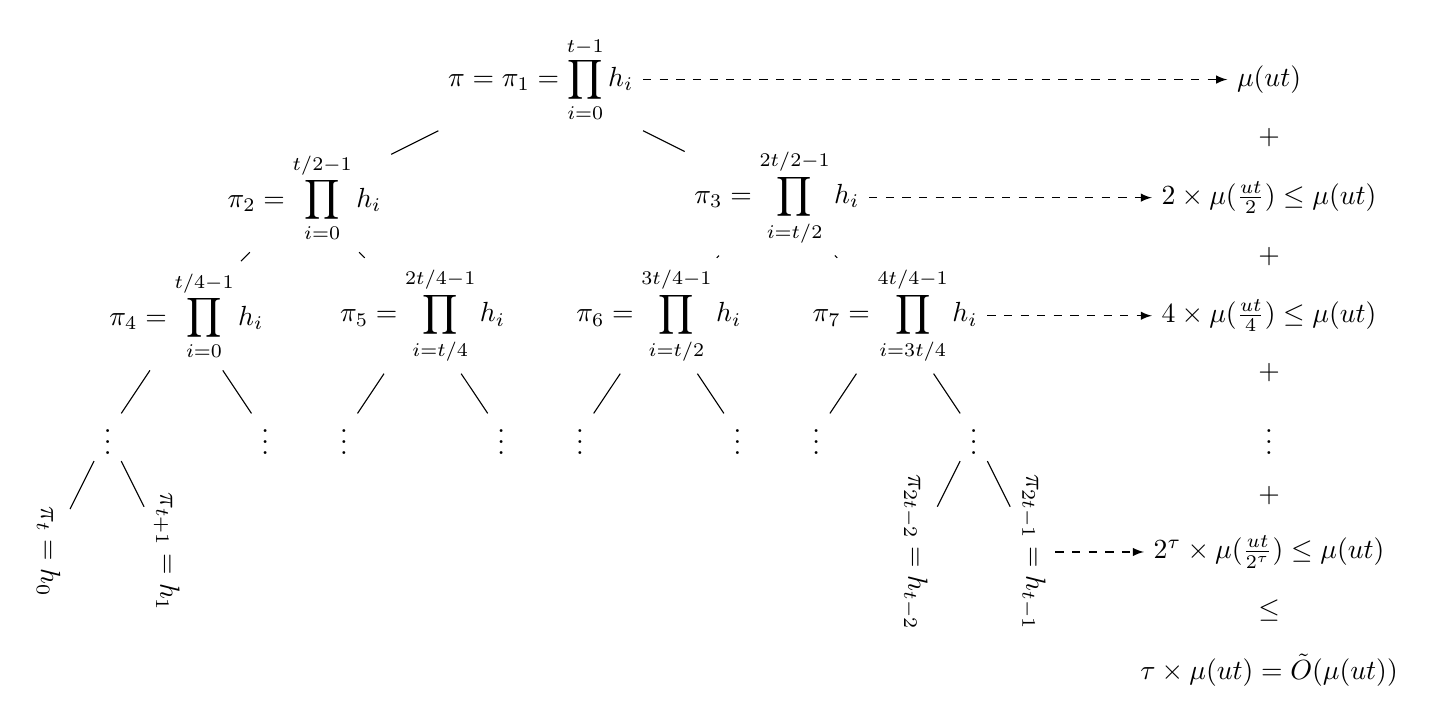
\begin{tikzpicture}[level/.style={sibling distance=60mm/#1}]
\node (z){$\displaystyle \pi=\pi_1=\prod_{i=0}^{t-1} h_i$}
  child {node (a) {$\displaystyle \pi_2=\prod_{i=0}^{t/2-1} h_i$}
    child {node (b) {$\displaystyle \pi_4=\prod_{i=0}^{t/4-1} h_i$}
      child {node {$\vdots$}
        child {node (d) {\begin{turn}{270}{$\displaystyle \pi_t=h_0$}\end{turn}}}
        child {node (e) {\begin{turn}{270}{$\displaystyle \pi_{t+1}=h_1$}\end{turn}}}
      }
      child {node {$\vdots$}}
    }
    child {node (g) {$\displaystyle \pi_5=\prod_{i=t/4}^{2t/4-1} h_i$}
      child {node {$\vdots$}}
      child {node {$\vdots$}}
    }
  }
  child {node (j) {$\displaystyle \pi_3=\prod_{i=t/2}^{2t/2-1} h_i$}
    child {node (k) {$\displaystyle \pi_6=\prod_{i=t/2}^{3t/4-1} h_i$}
      child {node {$\vdots$}}
      child {node {$\vdots$}}
    }
    child {node (l) {$\displaystyle \pi_7=\prod_{i=3t/4}^{4t/4-1} h_i$}
      child {node {$\vdots$}}
      child {node (c){$\vdots$}
        child {node (o) {\begin{turn}{270}{$\displaystyle \pi_{2t-2}=h_{t-2}$}\end{turn}}}
        child {node (p) {\begin{turn}{270}{$\displaystyle \pi_{2t-1}=h_{t-1}$}\end{turn}}
%
%
          child [grow=right] {node (qe) {} edge from parent[draw=none]
            child [grow=right] {node (q) {$2^\tau \times \mu(\frac{ut}{2^\tau}) \le \mu(u t)$} edge from parent[draw=none]
            child [grow=up] {node (r) {$\vdots$} edge from parent[draw=none]
            child [grow=up] {node (s) {$4\times\mu(\frac{u t}4) \le \mu(u t)$} edge from parent[draw=none]
            child [grow=up] {node (t) {$2\times\mu(\frac{u t}2) \le \mu(u t)$} edge from parent[draw=none]
            child [grow=up] {node (u) {$\mu(u t)$} edge from parent[draw=none]}
          }}}
          child [grow=down] {node (v) {$\tau \times \mu(u t) = \Oapp(\mu(u t))$}edge from parent[draw=none]}
            }
          }
        }
    }
  }
};
\path (q) -- (r) node [midway] {+};
\path (s) -- (r) node [midway] {+};
\path (s) -- (t) node [midway] {+};
\draw[->,>=latex,dashed] (l) to (s);
\path (t) -- (u) node [midway] {+};
\draw[->,>=latex,dashed] (z) to (u);
\draw[->,>=latex,dashed] (j) to (t);
\draw[->,>=latex,dashed] (p) to (q);
\path (q) -- (v) node [midway] {$\displaystyle \le$};
\end{tikzpicture}
\end{turn}
}
\caption{Product Tree}\label{fig:prod-tree}
\end{figure}

\begin{figure}
\centering
\centerline{
\begin{turn}{90}
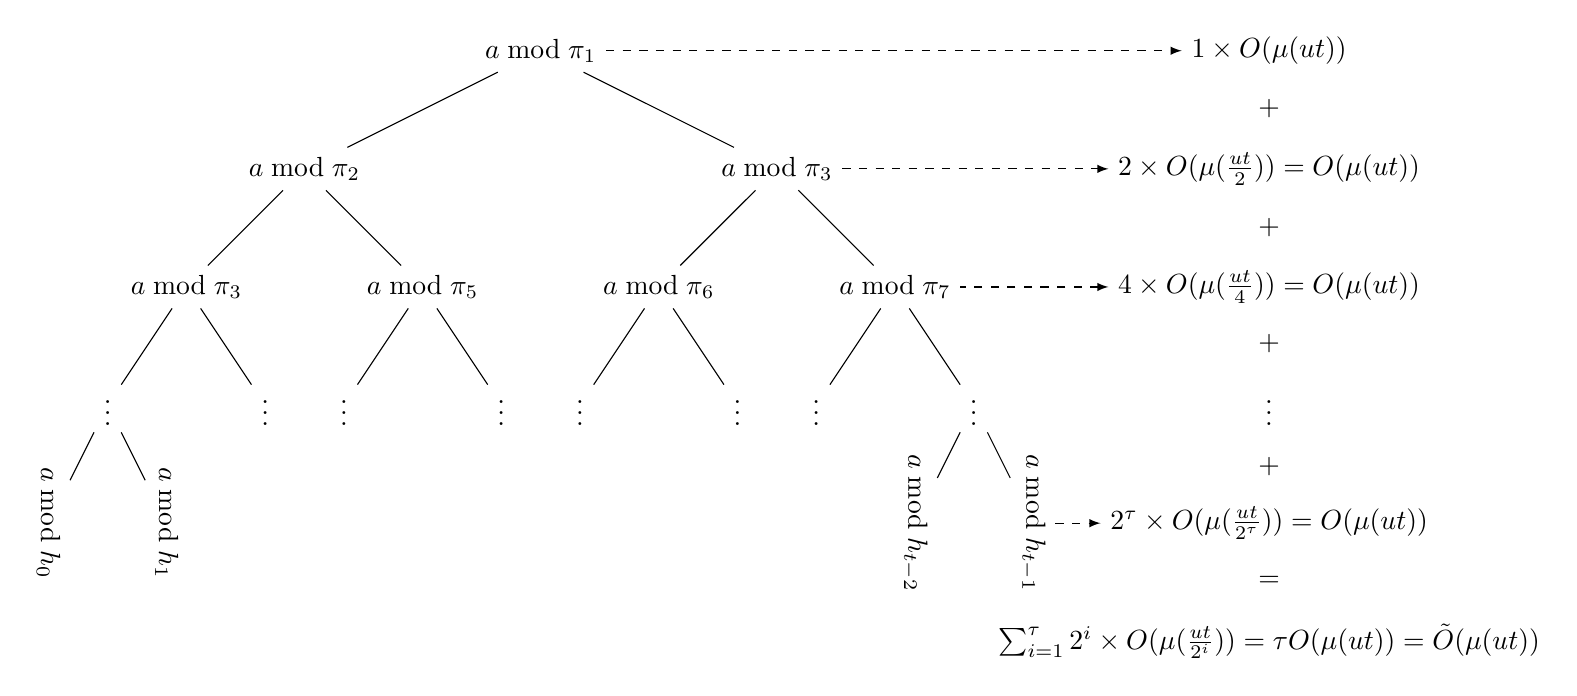
\begin{tikzpicture}[level/.style={sibling distance=60mm/#1}]
\node (z){$\displaystyle a \bmod \pi_1$}
  child {node (a) {$\displaystyle a \bmod \pi_2$}
    child {node (b) {$\displaystyle a \bmod \pi_3$}
      child {node {$\vdots$}
        child {node (d) {\begin{turn}{270}{$\displaystyle a \bmod h_{0}$}\end{turn}}}
        child {node (e) {\begin{turn}{270}{$\displaystyle a \bmod h_{1}$}\end{turn}}}
      }
      child {node {$\vdots$}}
    }
    child {node (g) {$\displaystyle a \bmod \pi_5$}
      child {node {$\vdots$}}
      child {node {$\vdots$}}
    }
  }
  child {node (j) {$\displaystyle a \bmod \pi_3$}
    child {node (k) {$\displaystyle a \bmod \pi_6$}
      child {node {$\vdots$}}
      child {node {$\vdots$}}
    }
    child {node (l) {$\displaystyle a \bmod \pi_7$}
      child {node {$\vdots$}}
      child {node (c){$\vdots$}
        child {node (o) {\begin{turn}{270}{$\displaystyle a \bmod h_{t-2}$}\end{turn}}}
        child {node (p) {\begin{turn}{270}{$\displaystyle a \bmod h_{t-1}$}\end{turn}}
%
%
          child [grow=right] {node (qe) {} edge from parent[draw=none]
            child [grow=right] {node (q) {$2^{\tau} \times O(\mu(\frac{ut}{2^{\tau}}))= O(\mu(u t))$} edge from parent[draw=none]
            child [grow=up] {node (r) {$\vdots$} edge from parent[draw=none]
            child [grow=up] {node (s) {$4 \times O(\mu(\frac{u t}4)) = O(\mu(u t))$} edge from parent[draw=none]
            child [grow=up] {node (t) {$2 \times O(\mu(\frac{u t}2)) = O(\mu(u t))$} edge from parent[draw=none]
            child [grow=up] {node (u) {$1 \times O(\mu(u t))$} edge from parent[draw=none]}
          }}}
          child [grow=down] {node (v) {$\sum_{i=1}^\tau 2^{i} \times O(\mu(\frac{ut}{2^i})) = \tau O(\mu(u t)) = \Oapp(\mu(u t))$}edge from parent[draw=none]}
            }
          }
        }
    }
  }
};
\path (q) -- (r) node [midway] {+};
\path (s) -- (r) node [midway] {+};
\path (s) -- (t) node [midway] {+};
\draw[<-,>=latex,dashed] (s) to (l);
\path (t) -- (u) node [midway] {+};
\draw[->,>=latex,dashed] (z) to (u);
\draw[->,>=latex,dashed] (j) to (t);
\draw[->,>=latex,dashed] (p) to (q);
\path (q) -- (v) node [midway] {$\displaystyle =$};
\end{tikzpicture}
\end{turn}}
\caption{Modular Reduction From Product Tree}\label{fig:div-prod-tree}
\end{figure}



\section{Implementation Details and Benchmarks}

Tables~\ref{tab:benchdirec}, \ref{tab:rsyncopt} and~\ref{tab:results}.

\begin{table}
\begin{center}
\begin{tabular}{ll}\toprule
~~{\bf Directory}              ~~&~~{\bf Description}\\\midrule
~~{\tt synthetic}              ~~&~~A directory containing 1000 very small files containing~~\\
~~                             ~~&~~the numbers $1,2,\ldots,1000$. \\
~~{\tt synthetic\_shuffled}    ~~&~~{\tt synthetic} with:\\
                             ~~& ~~~~~10 deleted files\\
                             ~~& ~~~~~10 renamed files \\
                             ~~& ~~~~~10 modified files \\
~~{\tt source}                 ~~& ~~A snapshot of \btrsync's own source tree \\
~~{\tt source\_moved}          ~~& ~~{\tt source} with one big folder (a few megabits) renamed.~~\\
~~{\tt firefox-13.0}           ~~& ~~The source archive of Mozilla Firefox 13.0.\\
~~{\tt firefox-13.0.1}         ~~& ~~The source archive of Mozilla Firefox 13.0.1\\
~~{\tt empty}                  ~~& ~~An empty folder.\\\bottomrule
\end{tabular}\smallskip
  \caption{Test Directories.}
  \label{tab:benchdirec}
\end{center}
\end{table}

\begin{table}
  \begin{tabular}{p{\dimexpr 0.25\linewidth-2\tabcolsep} p{\dimexpr
    0.75\linewidth-2\tabcolsep}}
    \toprule
    $\blacktriangleright$ {\tt --delete} & Delete existing files on Oscar which
    do not exist on Neil like \btrsync does.\\
    $\blacktriangleright$ {\tt -I} & Ensure that \rsync does not cheat by
    looking at file modification times (which \btrsync does not do).\\
    $\blacktriangleright$ {\tt --chmod="a=rx,u+w"} & Attempt to disable the
    transfer of file permissions (which \btrsync does not transfer). Although
    these settings ensure that \rsync does not need to transfer permissions,
    verbose logging suggests that it does transfer them anyway, so \rsync must
    lose a few bytes per file as compared to \btrsync for this
    reason.\\
    $\blacktriangleright$ {\tt -v} & Count the number of sent and received
    bytes. For \btrsync we added a piece of code counting the amount of data
    transmitted during \btrsync's own negotiations.\\
    \bottomrule
  \end{tabular}
  \caption{Options used when benchmarking \rsync}
  \label{tab:rsyncopt}
\end{table}

\comm{TODO: utiliser des préfixes SI pour une meilleure lisibilité}
\begin{table}
  \begin{tabular*}{\textwidth}{@{\extracolsep{\fill}}ll r r r r r r r r }
    \toprule
    \multicolumn{2}{c}{\bf Entities and Datasets} & \multicolumn{6}{c}{\bf Transmission (Bytes)} & \multicolumn{2}{c}{\bf Time (s)} \\
    \midrule {\bf \hfill Neil's $\mathfrak{F}'$ \hfill \null} & {\bf \hfill Oscar's $\mathfrak{F}$ \hfill \null}
    & $\mbox{{\tt TX}}_{\mbox{{\tiny {\tt rs}}}}$ & $\mbox{{\tt RX}}_{\mbox{{\tiny {\tt rs}}}}$  & $\mbox{{\tt TX}}_{\mbox{{\tiny {\tt bt}}}}$  & $\mbox{{\tt RX}}_{\mbox{{\tiny {\tt bt}}}}$  & $\delta_{\mbox{{\tiny {\tt rs}}}}-\delta_{\mbox{{\tiny {\tt bt}}}}$ &
    $\frac{\delta_{\mbox{{\tiny {\tt bt}}}}}{\delta_{\mbox{{\tiny {\tt rs}}}}}$ & $\mbox{{\tt time}}_{\mbox{{\tiny {\tt rs}}}}$ & $\mbox{{\tt time}}_{\mbox{{\tiny {\tt bt}}}}$ \\\midrule
    &&&&&&&&&\\[-1em]
    \texttt{source} & \texttt{empty} & 778311 & 1614 & 779517 & 10140 & 9732 & 1.0 & 0.1 & 0.4 \\
\texttt{empty} & \texttt{source} & 24 & 12 & 11927 & 5952 & 17843 & 496.6 & 0.1 & 0.4 \\
\texttt{empty} & \texttt{empty} & 24 & 12 & 19 & 30 & 13 & 1.4 & 0.0 & 0.3 \\
\texttt{synthetic} & \texttt{synthetic\_shuffled} & 54799 & 19012 & 7308 & 3417 & -63086 & 0.1 & 0.2 & 1.5 \\
\texttt{synthetic\_shuffled} & \texttt{synthetic} & 54407 & 18822 & 6822 & 3042 & -63365 & 0.1 & 0.2 & 0.8 \\
\texttt{synthetic} & \texttt{synthetic} & 54799 & 19012 & 327 & 30 & -73454 & 0.0 & 0.1 & 0.7 \\
\texttt{firefox-13.0.1} & \texttt{firefox-13.0} & 40998350 & 1187 & 39604079 & 3305 & -1392153 & 1.0 & 1.5 & 10.2 \\
\texttt{source\_moved} & \texttt{source} & 778176 & 1473 & 2757 & 1966 & -774926 & 0.0 & 0.1 & 0.6 \\

    \bottomrule
  \end{tabular*}

  \caption{Experimental results. {\tt rs} and {\tt bt} subscripts respectively denote {\tt rsync} and {\tt btrsync}. The two first columns indicate the datasets. Synchronization is performed \textit{from} Neil \textit{to} Oscar. {\tt RX} and {\tt TX} denote the quantity of received and sent bytes and $\delta_{\square}=\mbox{{\tt TX}}_{\square}+\mbox{{\tt RX}}_{\square}$. $\delta_{\mbox{{\tiny {\tt rs}}}}-\delta_{\mbox{{\tiny {\tt bt}}}}$ and ${\delta_{\mbox{{\tiny {\tt bt}}}}}/{\delta_{\mbox{{\tiny {\tt rs}}}}}$ express the absolute and the relative differences in transmission between the two programs. The last two columns show timing results. This evaluation was performed on an HP ProBook 5330m laptop using an Intel Core i3-2310M CPU clocked at 2.10 Ghz.}
  \label{tab:results}
\end{table}



\end{document}
